\chapter[Paper 2]{Periodic variability in the brightness of an ultra-hot Jupiter atmosphere}
\chaptermark{header title} %% if you want a different title in the headers
\label{ch4}

% Define the location of your plots
\graphicspath{{./gfx/Wasp18b/}}

% List all paper authors
\chauthors{Claire Baxter \&
          Jean-Michel D\'esert}

\chjournal{Astronomy \& Astrophysics, (to be submitted)}

\newcommand{\micron }{$\mu$m }
\newcommand{\CO}{\ce{CO}}
\newcommand{\water}{\ce{H2O}}
\newcommand{\methane}{\ce{CH4}}

\begin{abstract}
  % {} leave it empty if necessary
  \textit{Context} With close-in orbits and strong stellar irradiation on tidally locked daysides, hot Jupiter atmospheres are predicted to form large-scale weather structures. Observing the variability of a hot Jupiter is a key probe of such weather patterns as well as probing the atmospheric dynamics and temperature structures.\\
  % aims heading (mandatory)
  \textit{Aims} We aim to characterize the brightness variability of the ultra-hot Jupiter WASP-18b by analyzing ten secondary eclipses at 4.5~$\mu$m with Spitzer/IRAC.\\
  % methods heading (mandatory)
  \textit{Methods} Our observations span a time frame of 21.6 days which covers 23 planetary orbits. We search for temporal variability by robustly analyzing each of the lightcurves using our custom pipeline which implements pixel level decorrelation. We benchmark our results against the well-studied XO-3b.\\
  % results heading (mandatory)
  \textit{Results} We observe a variability in the eclipse depth with time, which is the first infrared temporal variability in secondary eclipse observations of hot Jupiters. Using a sinusoidal model, we derive a variability period of 23.12 $\pm$ 1.66 days and a peak-to-trough amplitude of 456 $\pm$ 71~ppm, corresponding to $\sim$12\% variability. We discuss possible causes of this variability, such as stellar variability, variable wind speeds, clouds, changes in atmospheric composition, and magnetic field coupling. We find that a 12\% variability signal would not be detected in the four available sectors of TESS containing WASP-18b, or with the 5 available HST/WFC3 eclipses, and that future observatories would be required for followup.
\end{abstract}

\section{Introduction}

Hot Jupiters are ideal targets for precise atmospheric characterization due to their large planet-to-star flux ratios. There have now been many secondary eclipse observations of hot Jupiters in the infrared, ranging from individual studies \citep[e.g.,][]{Charbonneau2005, Deming2005} to large-scale survey programs \citep[e.g.,][]{Schwartz2017, Baxter2020, Garhart2020}. The vast majority of hot Jupiter atmospheres are expected to form clouds and photochemical hazes \citep{Sing2016, Parmentier2016, Wakeford2019}. Inhomogeneous coverage of such clouds could lead to brightness variability in time.

Temporal variations have been observed at 5~$\mu$m in the equatorial banded structures of Jupiter \citep{Antunano2019}. Variability in time is also common in cool brown dwarfs, with variability amplitudes of a few percent in more than 50\% of L and T brown dwarfs \citep{Metchev2015}. Furthermore, variability has also recently been detected on directly imaged free-floating planetary-mass objects \citep[e.g.,][]{Biller2015}. However, observing variability on directly imaged exoplanets is difficult due to the contrast between the host star and planet \citep{Apai2016}.

%Variability in hot Jupiters.
Nevertheless, atmospheric variability in time has been measured with phase curve observations of 3 hot Jupiters to date: HAT-P-7b \citep{Armstrong2016}, Kepler-76b \citep{Jackson2019}, and WASP-12b \citep{Bell2019}. \citet{Armstrong2016} use 4 years of public \textit{Kepler} data of HAT-P-7b to search for variability. They find temporal variations in the phase curve shape, including the hot-spot offset, such that the hot-spot shifts from one side of the substellar point to the other on timescales of tens to hundreds of days. However, they find only marginal evidence of brightness variability in time, which they note can be explained by systematic noise in their fits. Also using \textit{Kepler} data, \citet{Jackson2019} found similar phase offset variability in Kepler-76b, however, they do measure variability in the phase curve amplitude. Furthermore, two phase-curve observations at 3.6~$\mu$m taken 3 years apart of WASP-12b measure the phase curve offset to be $32.6 \pm 6.2^{\circ}$ eastward to $13.6 \pm 3.8^{\circ}$ westward \citep{Bell2019}.

% HD189 paper
To date, there has been no periodic brightness variability measured in secondary eclipse observations of hot Jupiters in the infrared. \citet{Agol2010} place an upper limit of 2.7\% at 8~$\mu$m on the eclipse depth variability of HD 189733b. Furthermore, \citet{Kilpatrick2020} carried out multi-epoch secondary eclipse observations with Spitzer/IRAC in an attempt to constrain the variability of HD 189733b and HD 209458b. They do not find a periodic variability signal, but they can place upper limit constraints on any possible variability to 12\% and 1.6\% at 4.5~$\mu$m for HD 189733b and HD 209458b respectively.

% Causes of variability
A possible cause of the variability on HAT-P-7b in the optical is variable wind speeds leading to variable cloud coverage \citep{Armstrong2016}. Similarly, \citet{Jackson2019} proposed the advance and retreat of thermal structures on Kepler-76b. This leads to cloud formation on the nightside blowing over to the dayside and creating a feedback loop resulting in periodic variability. \citet{Rogers2017} explored the effect of magnetic fields on HAT-P-7b by incorporating magnetohydrodynamics (MHD) into their global circulation models (GCMs). They conclude that coupling of the magnetic field with ionized species in the atmosphere can act against the eastward hot spot offset caused by the day-night temperature contrast. Such feedback can settle into an oscillating pattern on timescales of $\sim10^6$ seconds, creating the observed variability. In the case of WASP-12b, analysis of the 3.6 and 4.5~$\mu$m phase curves suggest mass-loss of the planet \citep{Bell2019}. Variability in the mass loss rate could be the cause of the phase offset variability. However, they also note that, following the arguments of \citet{Rogers2017}, variability due to magnetic coupling would be expected on WASP-12b.

In this paper, we measure and discuss the atmospheric brightness variability in the infrared of the ultra-hot Jupiter WASP-18b.

\section{Observations}

We observed ten secondary eclipses of WASP-18b at 4.5~$\mu$m with Spitzer/Infrared array camera (IRAC), program 11099 (PI: Kreidberg). Each observation consisted of 11776 exposures of 2-second integration in sub-array mode, resulting in 6.54 hours per lightcurves. Our observations were preceded with a scheduled 30-minute throw-away "peak-up" observation to obtain accurate pointing before the main observation to minimize the effect of IRACs well known intrapixel sensitivity. The ten eclipses span from 8th-30th September 2015, a total time of 21.65 days, corresponding to 23 orbits of WASP-18b, given its orbital period of 0.94124000 days \citep{Pearson2019}.

Furthermore, we also analyzed the ten eclipses of XO-3b, program 90032 (PI: Knutson), to test the robustness of our pipeline and our results, particularly on the variability. These eclipses were previously part of the repeatability and reliability data challenge presented in \citet{Ingalls2016}.

\section{Data Analysis}

\subsection{Spitzer/IRAC photometric lightcurve reduction}

We reduce the Spitzer/IRAC secondary eclipse lightcurves with our custom pipeline described fully in Baxter et al. (submitted.) which follows the analysis method from \citep{Deming2015}. For clarity, we recall the main steps of our pipeline. In each of the Spitzer subarray frames, we correct the dark current, flat field, and convert to flux units before performing aperture photometry using a circular aperture around the calculated centroid position of the star. %We also calculate the midtimes of each photometric point from the UTC-based modified barycentric Julian date (MBJD) times in the file headers.
A full run of our pipeline creates a grid of data reductions and finds the optimum methods and parameters for background subtraction, centroiding, and aperture photometry radius utilizing a lowest reduced $\chi^2$ on the resulting lightcurves. Uncertainties on the photometric points are calculated from photon noise and scaled up such that the reduced $\chi^2$ after an initial least-squares fit is equal to 1.
%Our pipeline also removes some data from the beginning of the observation, we run a sequence of cuts to determine how much data to remove to minimize the reduced $\chi^2$ and the root mean square (RMS) of the residuals of the resulting lightcurve.

Our resulting optimum pipeline reduction methods were to centroid using the barycenter method, with a box size of 3x3, calculate the background using 4 pixels in each of the 4 corners of the image, and to perform aperture photometry with a radius of 2.5 pixels around the star. In each lightcurve, we masked between 0.053\% and 0.076\% bad pixels at 4$\sigma$. We also removed 15 minutes from the beginning of each of the lightcurves to remove the peak-up period of the observations. The best raw normalized photometric lightcurve for each observation is then used in the next step for a complete statistical analysis of the transit/eclipse parameters.

\subsection{Spitzer/IRAC secondary eclipse fitting}
\label{P3:sec:fitting}

To find the eclipse parameters from the raw photometric lightcurve, we fit a batman eclipse model \citep{Kreidberg2015} in combination with a temporal quadratic function (\nth{1} or \nth{2} order) and a pixel level decorrelation (PLD) systematic model \citep{Deming2015}. In our fit of WASP-18 b, we fix the period to 0.9414529 $\pm$ 0.00000234 \citep{Pearson2019} and the eccentricity and angle of periastron passage to 0.
% We also fix the parameters of a linear limb darkening law with limb darkening parameters calculated from the 1D ATLAS code presented in \citep{Sing2010} to 0.1601736 $\pm$ 0.00466754 at 4.5~$\mu$m. The stellar parameters use for this calculation were: 6400$\pm$100, 4.366$\pm$0.026, 0$\pm$0.1 for the effective temperature, surface gravity and metallicity respectively, taken from \citep{Southworth2009}.

Typically, the PLD systematic model uses a 3x3 grid of pixels around the centroid of the star to model the systematics. Since WASP-18b is a bright star, a significant portion of the stellar PSF may spread beyond these nine pixels, we, therefore, test the effect of including more pixels with a 5x5 PLD grid. However, we found that a 5x5 PLD box compared to a 3x3 PLD box was not improving the fits.
%necessary as it resulted in overfitting (mean $\Delta$BIC over 10 lightcurves is -960).

Furthermore, since assuming a \nth{1} order quadratic (linear) baseline can result in underestimating the eclipse depth for hot planets with large phase amplitudes \citep[e.g.,][]{Bell2019}, we also tested a \nth{2} order quadratic baseline in time. However, such a \nth{2} order quadratic coefficient can also be degenerate with the eclipse depth. We tested including a \nth{2} order quadratic baseline (2 free parameters) compared to a \nth{1} order baseline (1 free parameter). We found that it was not statistically significant to have a \nth{2} order quadratic free in each of the fits (mean $\Delta$BIC of 3). However, we also tested fixing the \nth{2} order quadratic co-efficient while still leaving the \nth{1} order co-efficient free. This test was statistically significant (mean $\Delta$BIC of 53) when comparing it with a \nth{1} order quadratic (linear) baseline. We, therefore, opted to fix the \nth{2} order coefficient to the weighted mean value from the first fit, -0.031 $\pm$ 0.004. This method corrects the astrophysical signal from the large phase amplitudes (\nth{2} order) without compromising the systematic correction (\nth{1} order) and thus leads to accurate results on the eclipse depths.

To achieve our final results we perform two fits of the lightcurves. First, we perform an initial fit with 15 free parameters ($a/R_s$, inclination, $F_p/F_s$, $T_{secondary}$, 9 PLD parameters and a \nth{2} order quadratic baseline in time). Then we fix $a/R_s$, inclination and the \nth{2} order quadratic coefficient to the weighted mean over all ten lightcurves. We do this since we do not expect these parameters to be physically changing in time. Our final MCMC fits have 12 free parameters ($R_p/R_s$, $T_{secondary}$, 9 PLD parameters and 1 temporal slope). As a sanity check, we compare the brightness temperatures between the first and second fit in Figure \ref{P3:app:depths}, and find that it still shows variability.

Posterior distributions and uncertainties are calculated on the fitted parameters by performing a full Markov Chain Monte Carlo (MCMC) exploration of parameter space using emcee \citep{Foreman-Mackey2013}. We run chains with 100 walkers with a typical 500 step burn-in period followed by a 1000 step production run and confirm the convergence of our chains via the auto-correlation time and the mean acceptance fraction.

\section{Results}
\subsection{Spitzer/IRAC secondary eclipse lightcurves}
\label{P3:sec:lcresults}

Table \ref{P3:tab:resutls} displays the $a/R_s$, inclination and \nth{2} order quadratic coefficient from the first fit alongside
% We do not find any variability in $a/R_s$ and inclination with time, so we fix these parameters to the weighted mean for the second fit. Additionally, we find that the \nth{2} order quadratic coefficient is degenerate with the eclipse depth and results in a worse BIC, so we also fix this to the weighted mean as mentioned in Section \ref{P3:sec:fitting}.
$F_p/F_s$, $T_{secondary}$ and $T_B$ from the second fit. Figure \ref{P3:fig:correctedlcs} shows the final resulting systematic corrected lightcurves. We find that the weighted mean eclipse depth is 3729 $\pm$ 56~ppm, which is consistent with the eclipse presented in \citet{Nymeyer2011} and the phase curve presented in \citet{Maxted2013}. We also find that the weighted mean secondary eclipse timings are within 1$\sigma$ agreement with the previously calculated eclipse ephemeris from \citet{Maxted2013}. Raw lightcurves and residuals are shown in Appendix \ref{P3:app:plots}.

\begin{figure}
    \centering
    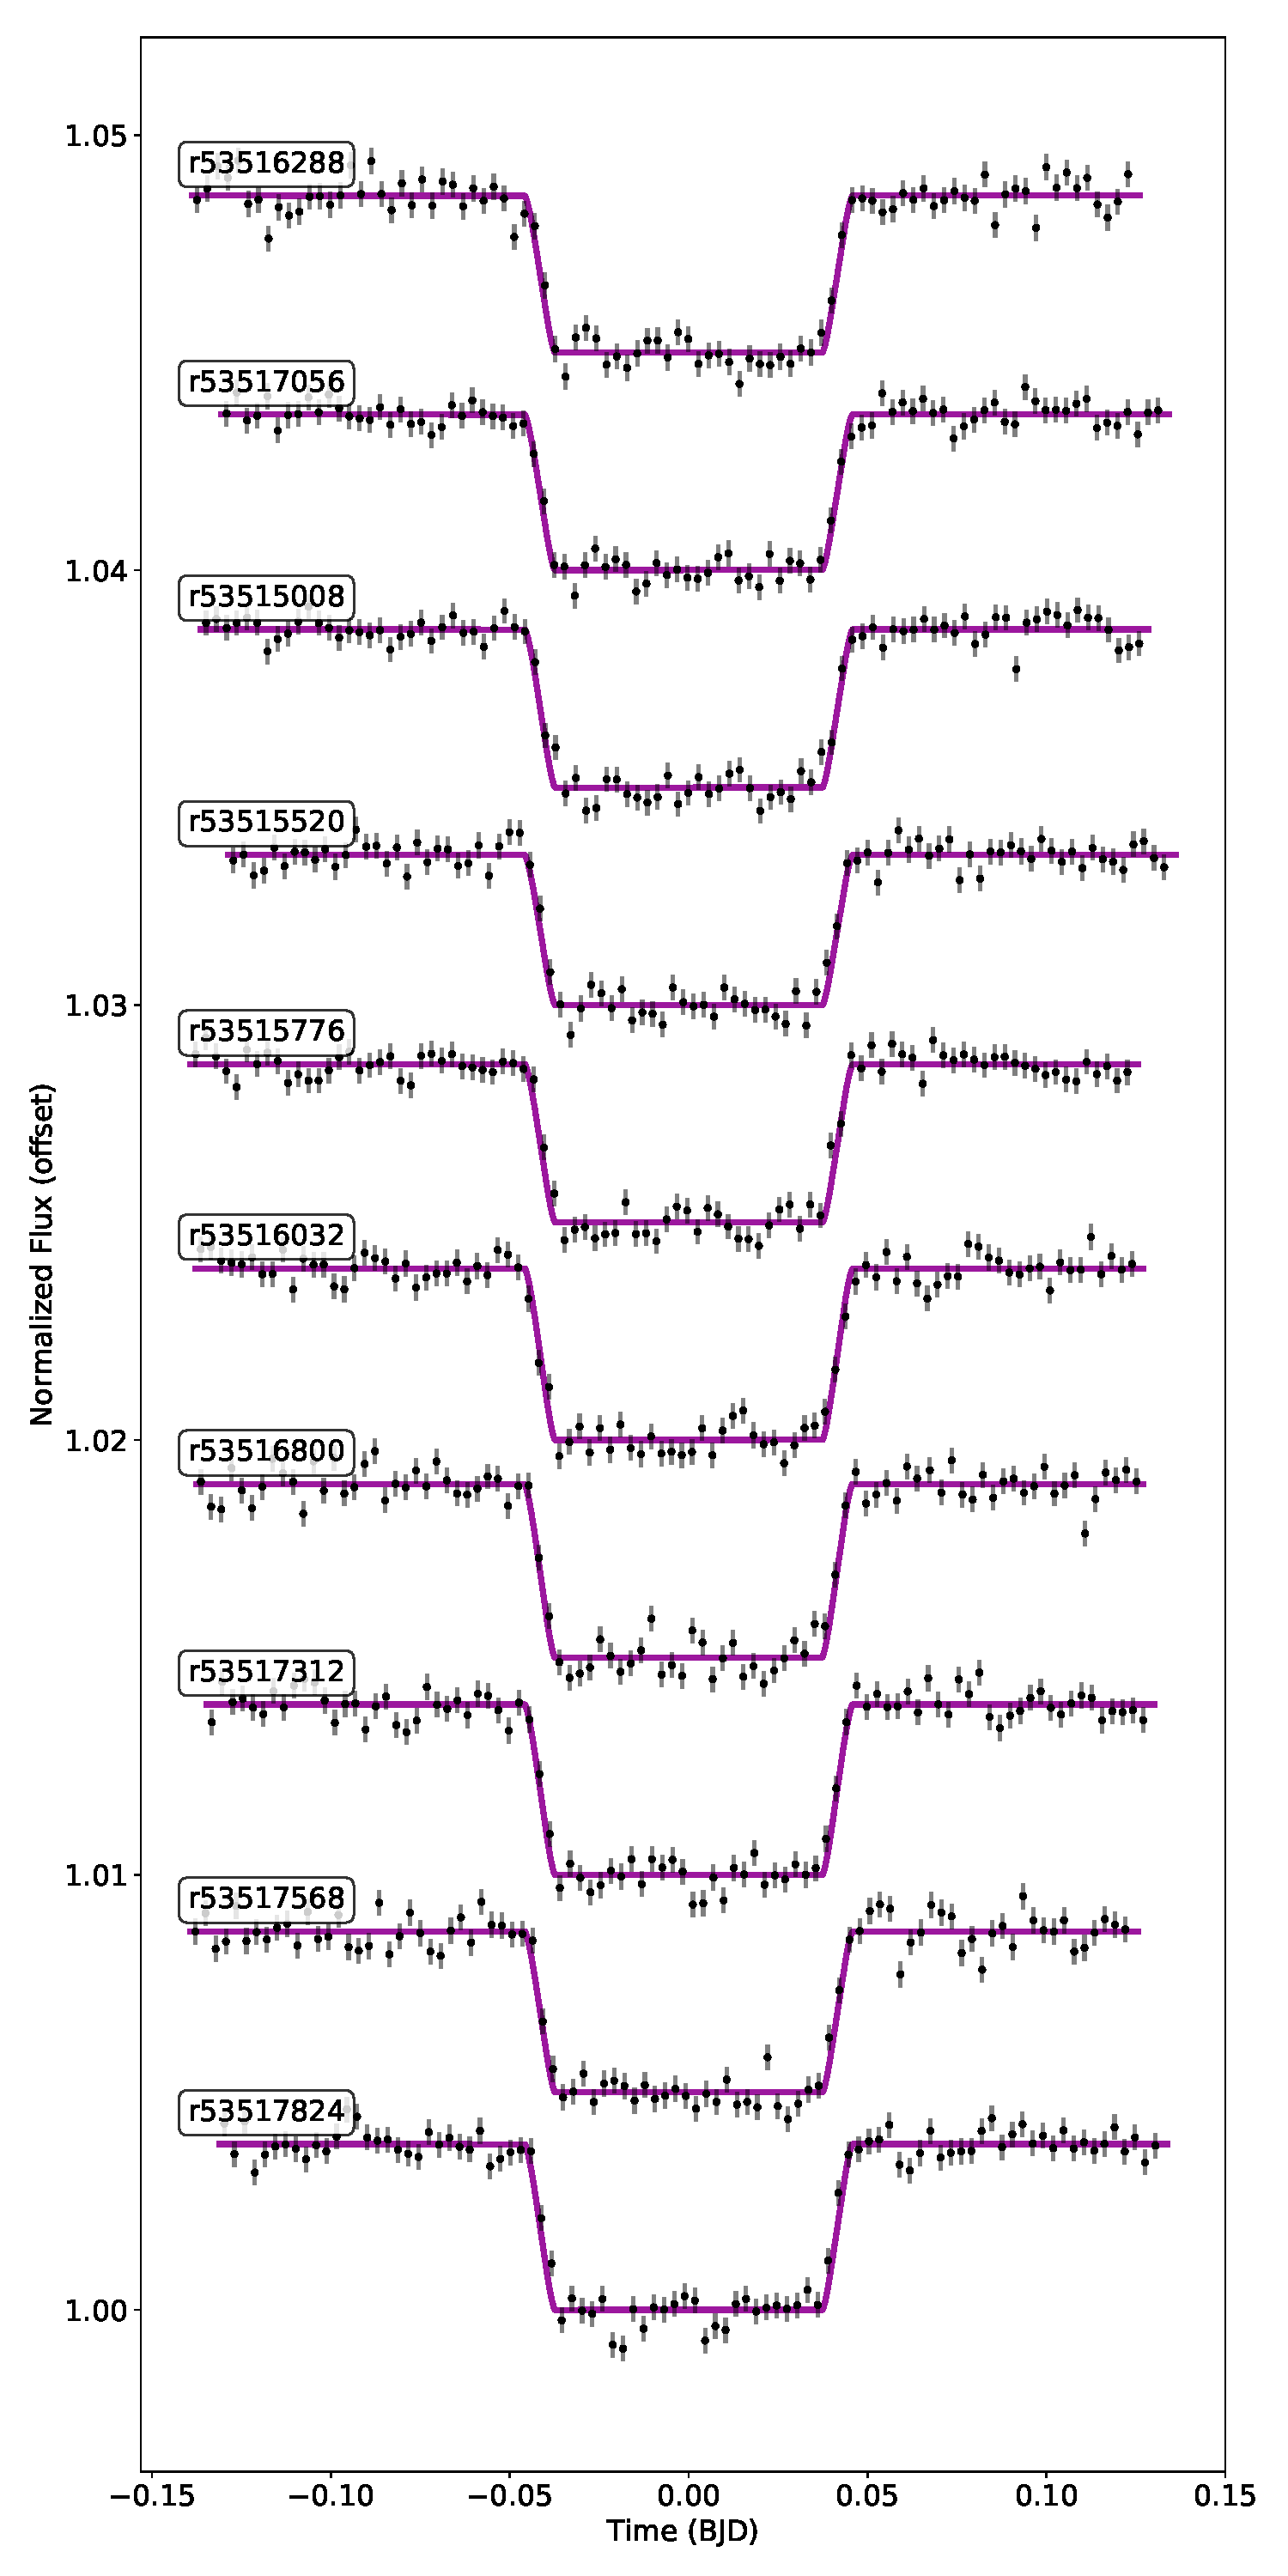
\includegraphics[height=\textheight]{Correctedlightcurves_W18b.pdf}
    \caption{Normalized and corrected eclipse lightcurves of WASP-18b, vertically offset for display purposes. These lightcurves are from the final fit, where we fixed $a/R_s$, inclination and the \nth{2} quadratic coefficient to their weighted means from the first fit. }
    \label{P3:fig:correctedlcs}
\end{figure}

\begin{landscape}
\begin{table*}[]
    \centering
    \caption{Best fit eclipse and systematic parameters using an MCMC method. The semi-major axis ($a/R_s$), inclination and 2nd order quadratic co-efficient (h) are shown from the first fits, they are fixed to the weighted mean in the final fit. The eclipse depth ($F_p/F_s$), brightness temperature ($T_B$) and the time of secondary eclipse ($T_{secondary}$) are shown from the final fits.}
    \label{P3:tab:resutls}
\begin{tabular}{lccc|ccc}
\hline \hline
 AOR & $a/R_s$ & Inclination & h & $F_p/F_s$ & $T_B$ & $T_{secondary}$ \\
 &  & Degrees & &~ppm & Kelvin & BJD \\
\hline
r53517824 & 3.48 $\pm$ 0.15 &  83.29 $\pm$ 2.05 &   -0.03 $\pm$ 0.008 &  3810 $\pm$ 68 &  3079 $\pm$ 37 &  2457274.14104 $\pm$ 0.00029 \\
r53517568 & 3.46 $\pm$ 0.14 &  83.38 $\pm$ 1.95 &  -0.039 $\pm$ 0.008 &  3700 $\pm$ 68 &  3011 $\pm$ 37 &   2457275.08202 $\pm$ 0.0003 \\
r53517312 & 3.43 $\pm$ 0.16 &  83.09 $\pm$ 2.22 &   -0.035 $\pm$ 0.01 &  3919 $\pm$ 78 &  3166 $\pm$ 41 &  2457278.84855 $\pm$ 0.00028 \\
r53516800 & 3.34 $\pm$ 0.15 &  82.04 $\pm$ 1.94 &  -0.038 $\pm$ 0.008 &  3984 $\pm$ 66 &  3163 $\pm$ 36 &  2457279.78877 $\pm$ 0.00026 \\
r53516032 & 3.15 $\pm$ 0.15 &  80.42 $\pm$ 1.75 &  -0.011 $\pm$ 0.009 &  3954 $\pm$ 69 &  3147 $\pm$ 37 &  2457283.55482 $\pm$ 0.00028 \\
r53515776 & 3.48 $\pm$ 0.14 &  83.27 $\pm$ 1.85 &  -0.041 $\pm$ 0.008 &  3640 $\pm$ 68 &  2984 $\pm$ 38 &  2457286.37946 $\pm$ 0.00028 \\
r53515520 & 3.28 $\pm$ 0.18 &  81.15 $\pm$ 2.26 &  -0.046 $\pm$ 0.009 &  3454 $\pm$ 70 &  2890 $\pm$ 37 &  2457288.26257 $\pm$ 0.00029 \\
r53515008 & 3.06 $\pm$ 0.18 &   78.70 $\pm$ 2.09 &  -0.028 $\pm$ 0.009 &  3633 $\pm$ 67 &  2988 $\pm$ 35 &   2457289.2035 $\pm$ 0.00029 \\
r53517056 & 3.32 $\pm$ 0.19 &  82.08 $\pm$ 2.41 &  -0.025 $\pm$ 0.008 &  3585 $\pm$ 71 &  2943 $\pm$ 37 &  2457293.91153 $\pm$ 0.00031 \\
r53516288 & 3.38 $\pm$ 0.18 &  82.32 $\pm$ 2.27 &  -0.013 $\pm$ 0.009 &  3616 $\pm$ 69 &  2973 $\pm$ 38 &   2457295.79433 $\pm$ 0.0003 \\
\hline
Weighted Mean & 3.45 $\pm$ 0.04 & 81.96 $\pm$ 0.49 & -0.031 $\pm$ 0.004 & 3729 $\pm$ 56 & 3033 $\pm$ 31 & \\
\hline
Standard Deviation & 0.13 & 1.43 & 0.01 & 169 & 93 & \\
Mean Error & 0.16 & 2.08 & 0.01 & 69 & 37 & \\
\hline
\end{tabular}

\end{table*}
\end{landscape}

\subsection{Brightness variability of WASP-18b in time}

% Compare to a straight line.
We plot the secondary eclipse depths of WASP-18b in time (see Figure \ref{P3:fig:variability}), and we find that the eclipse depths are not constant, but instead they show a level of variability, that isn't random, but that is reproduced by a periodic sinusoidal signal. We find that the eclipse depth measurements deviate from a straight line by more than 7$\sigma$. We fit this temporal brightness variability with a sinusoidal function in time (t).
%We parameterize the sinusoid with three free parameters: amplitude (A), frequency ($\nu$) and an offset ($\bar{D}$). We tested having an additional phase parameter ($\varphi$) but this did not significantly improve the fits ($\Delta$BIC = 2.2). Therefore, we fixed phase to zero such that the eclipse depths in time are modeled by the following equation: D = Asin($\nu$t) + $\bar{D}$.
We parameterize the sinusoid with four free parameters: semi-amplitude ($A$), frequency ($\nu$), phase ($\varphi$) and an offset ($\bar{D}$) such that the eclipse depths in time are modeled with $D(t)$ = $A$sin($\nu$t) + $\bar{D}$. We tested fixing the phase parameter ($\varphi$) but this did not significantly improve the fits ($\Delta$BIC = 2.2).
We calculate posterior distributions on these parameters by running an MCMC exploration using emcee \citep{Foreman-Mackey2013} with 300 walkers, 1000 burn-in steps and 20000 production steps. We confirm convergence of the chains using the auto-correlation time and the mean acceptance fraction. We then test the robustness of our sinusoidal fit by comparing it with a straight line using the Bayesian Information Criteria (BIC).

Figure \ref{P3:fig:MCMCcorner} shows the posterior distributions from the MCMC sinusoidal fits and the best sinusoidal fit is also shown in Figure \ref{P3:fig:variability}. We find that the sinusoidal fit is statistically significantly favored over a straight line fit where BIC of the straight line being 62.3 and the BIC of the sinusoid being 18.2.
% The best fit sinusoidal parameters are: A = -0.00023 $\pm$ 3.5e-05, $\nu$ = 0.27 $\pm$ 0.019, $\varphi$ = 3.1 $\pm$ 0.23, $\bar{D}$ = 0.0037 $\pm$ 2.3e-05. This corresponds to a 23.16 $\pm$ 1.73 days period of variability and a 228.39 $\pm$ 35.23~ppm amplitude of variability. The weighted mean eclipse depth of all 10 eclipses results in an eclipse depth of 3725 $\pm$ 57~ppm, meaning the measured variability amplitude is 6.1$\pm$0.9\%.
The best fit sinusoidal parameters are: $A$ = 228$\pm$36~ppm, $\nu$ = 0.27$\pm$0.02, $\varphi$ = -0.01$\pm$0.23, $\bar{D}$ = 3732$\pm$23~ppm. This corresponds to a 23.1$\pm$1.7 days period of variability and a 12.2$\pm$1.9\% peak-to-trough brightness variability (2$A$).

We tested for variability and correlations with the other parameters we let free in the fits. The standard deviation is smaller than the mean error over all ten lightcurves for $a/R_s$ and inclination (see Table \ref{P3:tab:resutls}. This indicates that there is no variability in these parameters. We also tested for correlations between $a/R_s$ and inclination with $F_p/F_s$, in both cases they had low Pearson correlation coefficients (0.05 and 0.13 respectively) with high associated chance probabilities (0.9 and 0.7 respectively). These numbers indicate that $a/R_s$ and inclination are not correlated with $F_p/F_s$.

\begin{sidewaysfigure}
    \centering
    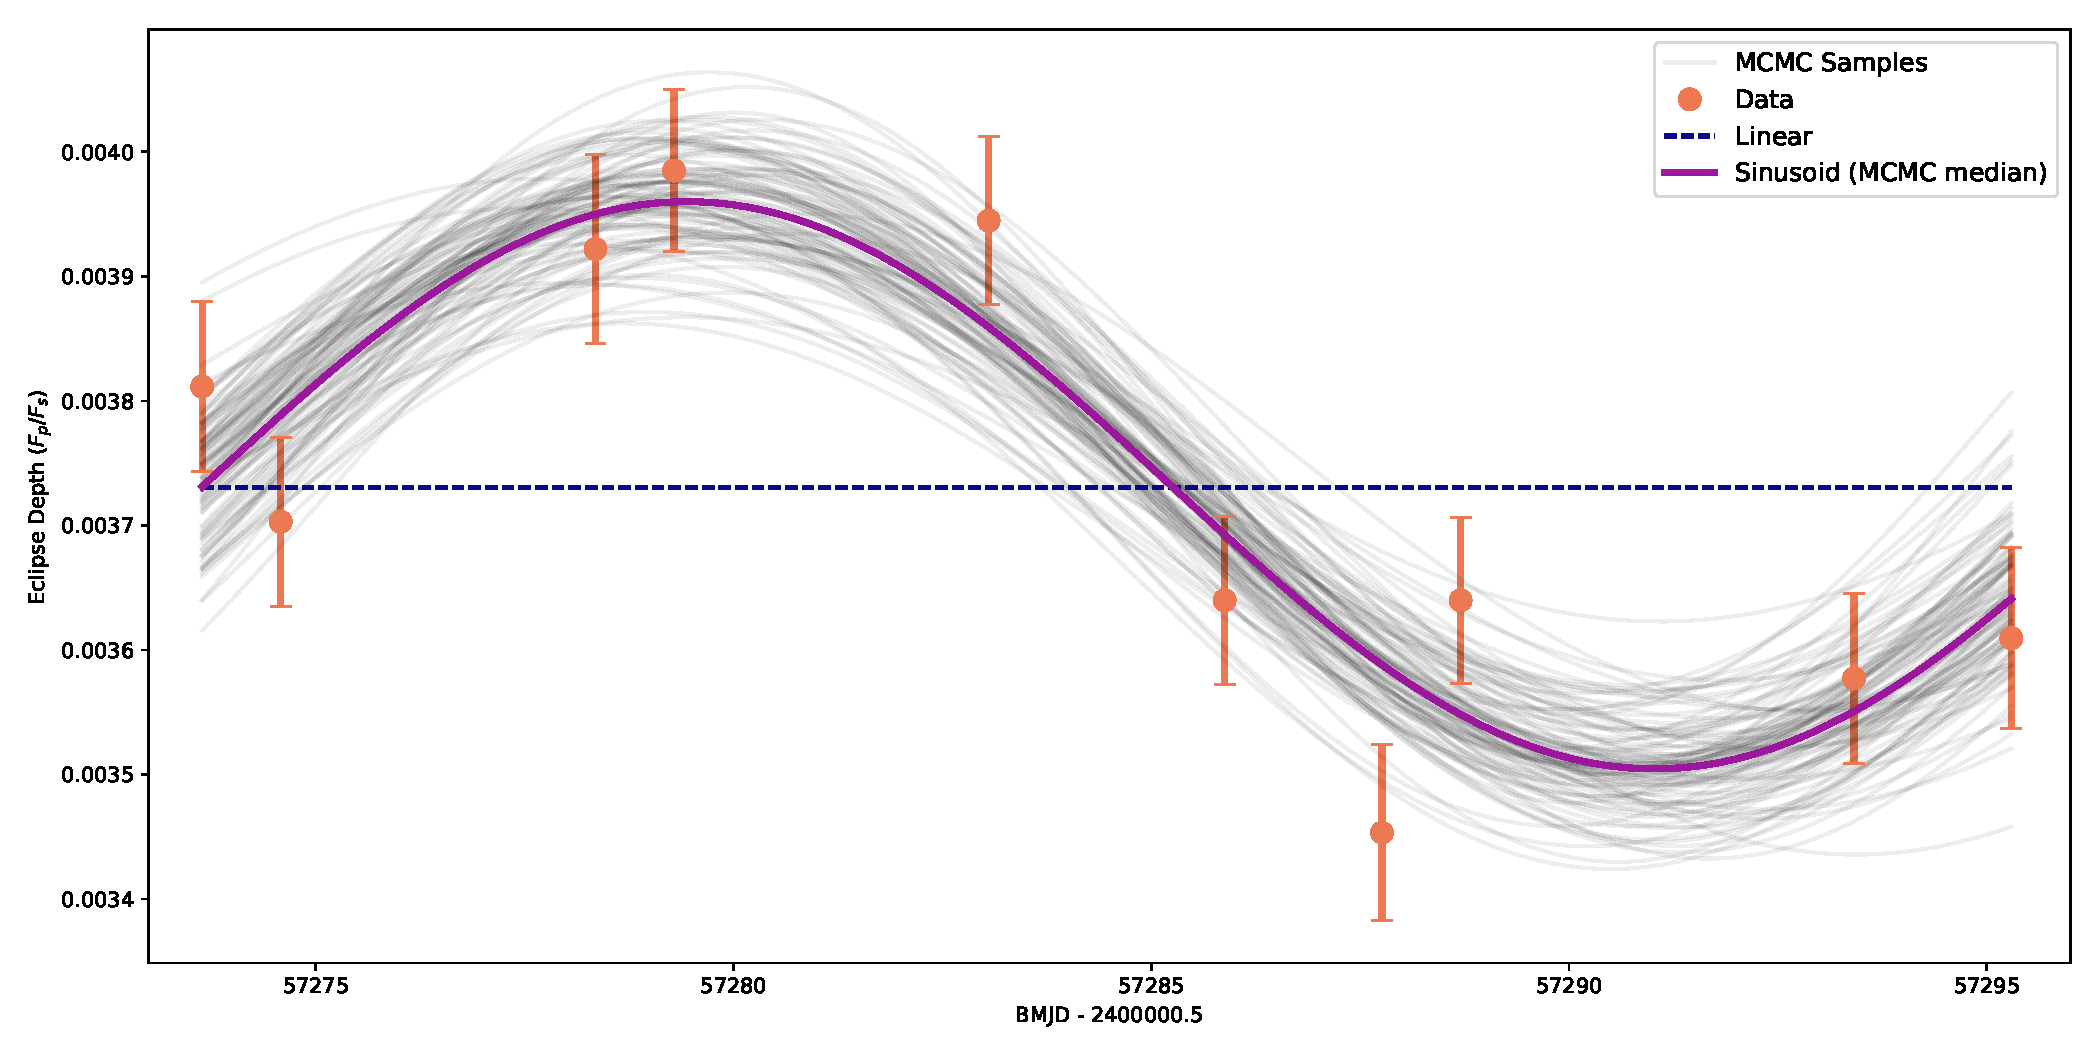
\includegraphics[width=\linewidth]{MCMCvarsamples.pdf}
    \caption{Measured eclipse depths of WASP-18b over time in orange, for the ten semi-consecutive eclipses. Purple solid line shows the median result from the MCMC fit, 100 random samples from the posterior distributions are shown in gray, blue line shows the best fitting straight line.}
    \label{P3:fig:variability}
\end{sidewaysfigure}

\begin{figure}
    \centering
    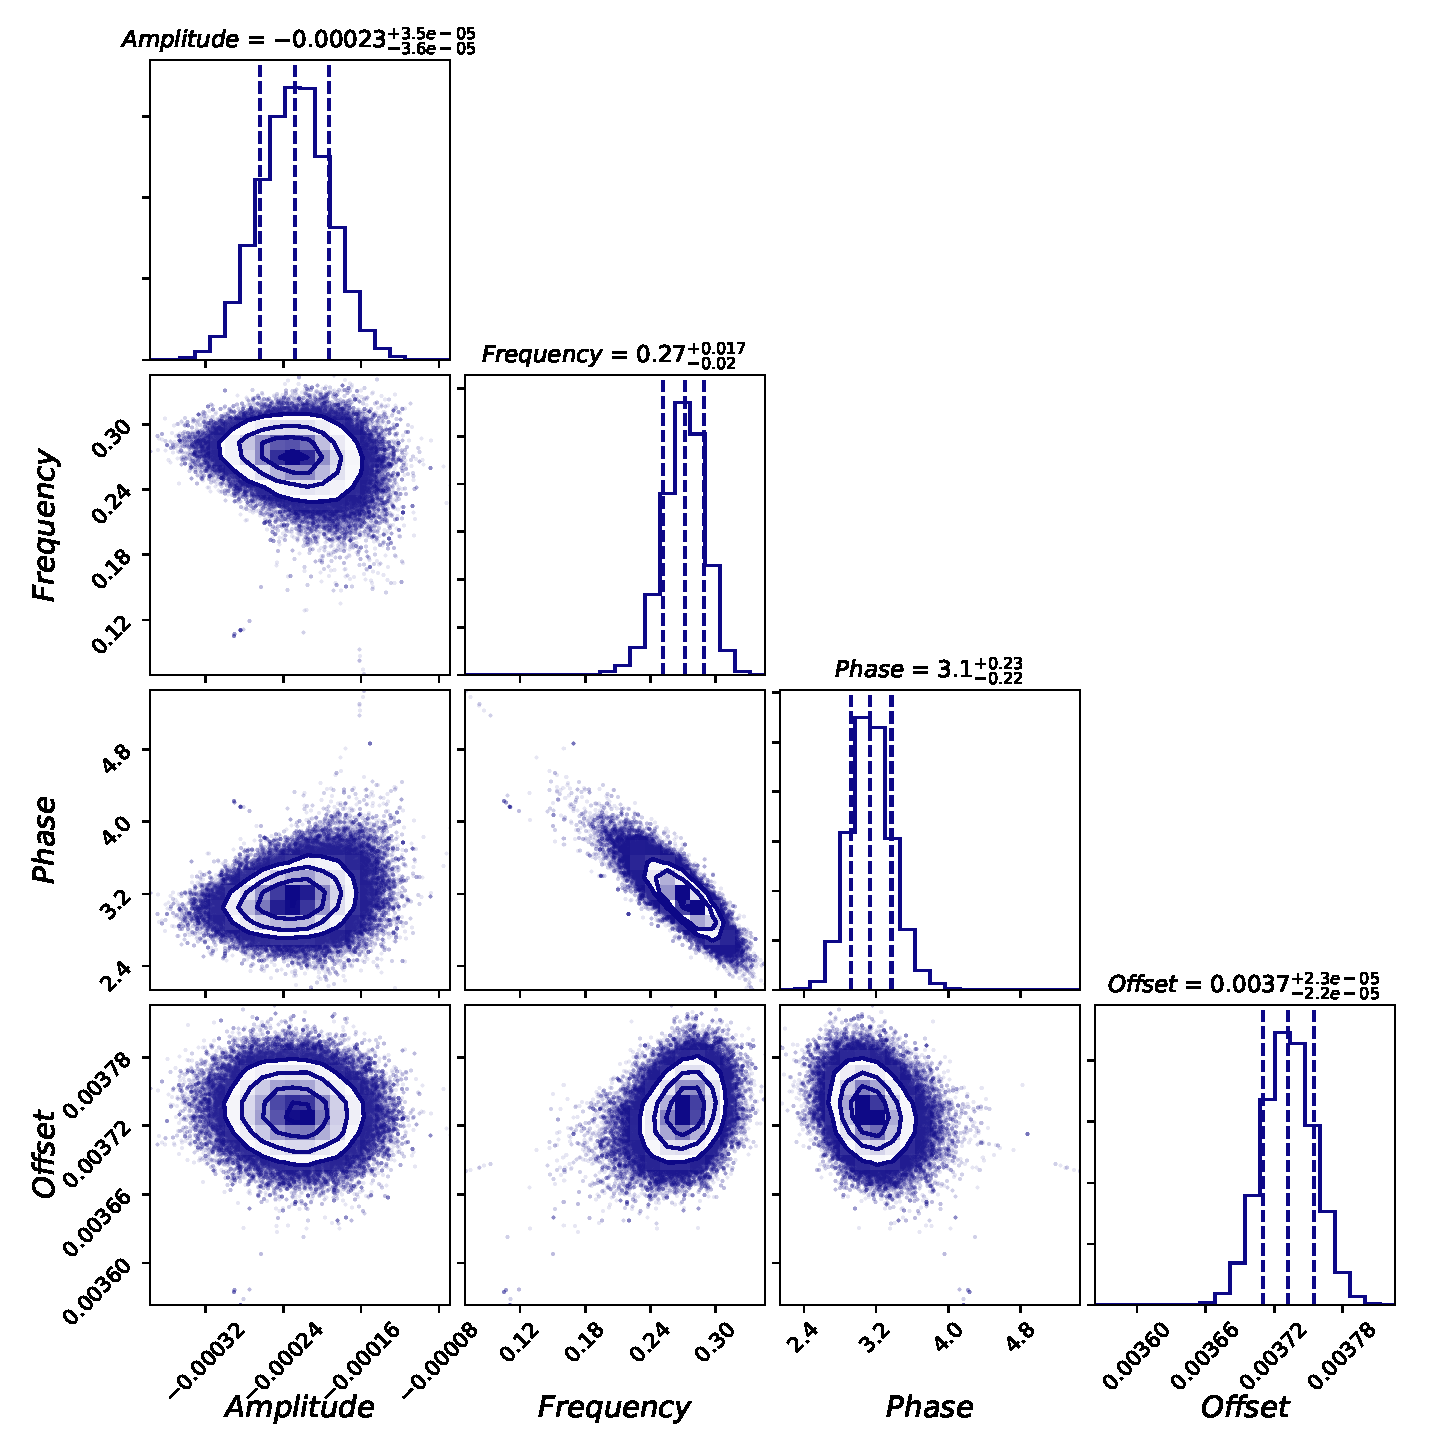
\includegraphics[width=\linewidth]{MCMCcorner.pdf}
    \caption{Posterior probability distributions of the free parameters from a periodic sinusoidal MCMC fit to the brightness variability in time of WASP-18b at 4.5~$\mu$m. In the marginalized confidence intervals the inner dashed line is the median and the outer dashed lines are the 1$\sigma$ confidence level. }
    \label{P3:fig:MCMCcorner}
\end{figure}

\subsection{Testing the method to measure variability}

To test the robustness of our analysis and ensure that our method does not introduce any spurious variability, we analyze the ten secondary eclipses of another hot Jupiter, XO-3b, which has been widely studied, and which serves as a calibration of our methods. These eclipses were first published in \citet{Wong2014} and later used as part of the extensive repeatability and accuracy post-cryogenic Spitzer/IRAC data challenge \citep{Ingalls2016}. \citet{Ingalls2016} test seven different techniques for correcting the correlated noise. Across these seven techniques they measure an average eclipse depth of $1520 \pm 30$~ppm. This value is a straight average of the weighted mean and weighted uncertainty over the ten eclipses for each technique. We calculate the weighted mean and weighted uncertainty using the same method (see their eq. 5-9) and find that the weighted mean eclipse depth of our PLD corrected secondary eclipses to be $1520 \pm 29$~ppm. This is in remarkable agreement with \citet{Ingalls2016} and we conclude that our pipeline produces consistent results.

For XO-3b we measure the mean uncertainty over the ten eclipses to be 84~ppm, which is in agreement with the average precision achieved over the seven different techniques in \citet{Ingalls2016}, which was 102~ppm (ranging from 48~ppm to 152~ppm). We also find that the standard deviation of the ten eclipse depths to be 86~ppm. The fact that the mean uncertainty and the standard deviation are the same indicates that the eclipse depths are drawn from a random distribution, and there is no evidence for variability in the eclipses of XO-3b. On the other hand, for WASP-18b, the mean uncertainty of the ten eclipse depths is 69~ppm, yet the standard deviation is 173~ppm. This indicates that there is variability measured at a significant level in the secondary eclipse measurements of WASP-18b.

\subsection{Variability of WASP-18b at various wavelengths}

WASP-18b was also observed at 3.6~$\mu$m with Spitzer/IRAC on two occasions: an eclipse was observed in December 2008, $F_p/F_s$=3040$\pm$170~ppm \citep{Nymeyer2011}, and a phase curve was observed in January 2010, $F_p/F_s$=3000$\pm$200~ppm \citep{Maxted2013}. These two eclipse depths are consistent to within 1$\sigma$ and so cannot rule out or confirm variability at 3.6~$\mu$m.

\citet{Shporer2019} measure the eclipse depth of WASP-18b with 40 TESS eclipses to be $341^{+17}_{-18}$~ppm. A $\sim$12\% variability in TESS would result in a 21~ppm variability semi-amplitude. The precision on one eclipse measured with TESS would be $18\times\sqrt{N}$, where N is the number of measurements, resulting in a precision of 113~ppm on each eclipse. Using this precision, we simulate the 40 individual eclipses from Sectors 2 and 3 in \citet{Shporer2019} and the 58 additional unpublished eclipses from Sectors 29 and 30. We then add a 21~ppm sinusoidal variability signal and try to retrieve it using MCMC. We find that TESS does not have the precision to detect the 21~ppm variability to greater than 1$\sigma$ with the 98 simulated eclipses.

Furthermore, \citet{Arcangeli2018} publish 5 secondary eclipses of WASP-18b with HST/WFC3. Their combined spectrum is measured to $\sim$20~ppm precision per bin. Using this, we calculated the precision on the combined white lightcurve to be 38~ppm. This means that the precision on one eclipse is 45~ppm per bin and 86~ppm on the white lightcurve. A $\sim$12\% peak-to-trough variability would result in 46-72~ppm semi-amplitudes over the spectral range. Using the same method as above, we found that HST/WFC3 does not have the precision to detect this variability across 5 eclipses in either the white light curve or the individual bins.

\section{Discussion \& Conclusion}

% \begin{itemize}
%     \item Stellar variability
%     \begin{itemize}
%         \item Less in infrared than optical
%         \item WASP-18 has low activity index (Fossati 2018)
%     \end{itemize}
%     \item Formation of clouds
%     \begin{itemize}
%         \item Wasp-18b is probably too hot for clouds
%         \item only on western terminator (Helling 2019)
%     \end{itemize}
%     \item Compositional variability in time
%     \begin{itemize}
%         \item Unlikely what we are seeing since 4.5 micron is sensitive to CO which is not sensitive to these temperature differences
%     \end{itemize}
%     \item Magnetic field coupling
%     \begin{itemize}
%         \item Alfven waves - timescale scaling to HAT-P-7b
%     \end{itemize}
%     \item Star-planet interactions
%     \begin{itemize}
%         \item link to magnetic fields and dissipation/play off between these two effects
%     \end{itemize}
%     \item Do I need a conclusion section?
% \end{itemize}

% We explore the various possible origins of the variability measured at 4.5~$\mu$m below. This includes brightness temperature and compositional variations, clouds, effects of magnetic field and stellar variability.

% Intro sentence
We explore the possible origins of the variability in the dayside of an ultra-hot Jupiter atmosphere, these are: changes in disk-integrated temperature, compositional changes, the presence of inhomogeneous clouds, magnetic field interactions or stellar variability.

% Changes in TP and changes in Composition
We first consider whether the periodic change in eclipse depths measured at 4.5~$\mu$m could be due to variability of the atmosphere of the planet itself. Variability in the eclipse depths relates directly to variability in the disc averaged brightness temperatures (see Table \ref{P3:tab:resutls}). The peak-to-trough change in the brightness temperature of our sinusoidal fit is $\sim$250~K. GCMs of WASP-18b show that the temperature pressure profiles on the dayside change significantly from the coolest western terminator to the hottest substellar point \citet{Helling2019b}. At the millibar level, which corresponds to the pressures probed by Spitzer, these temperatures change by almost 1000~K. 250~K variability in the disc averaged temperature could lead to compositional variability in the atmosphere in time. However, the dominating opacity at the 4.5~$\mu$m band of Spitzer/IRAC is carbon monoxide and the abundance weighted opacity is relatively constant, even over the 1000~K temperature gradient spanned by the hot spot to the western terminator \citep[e.g.,][]{Moses2013}. It is therefore unlikely that we are detecting changes in the volume mixing ratio of CO at 4.5~$\mu$m.

% H2 dissociation/recombination
However, high levels of \ce{H2} dissociation are expected in the atmospheres of UHJs, atomic hydrogen can be transported to the nightside via eastward winds where it recombines and deposits a large amount of heat \citep{Komacek2018, Bell2018}. Given a fixed wind speed, this will increase the global efficiency of heat redistribution. However, if the wind speeds are variable, the heat re-circulation from \ce{H2} dissociation/recombination will also vary, and so might the measured brightness.

% Clouds
A second possible cause of variability in the atmosphere of WASP-18b is the presence of clouds. A previous theoretical study has examined cloud formation on WASP-18b using GCMs \citep{Helling2019b}. They extract 1D profiles to use as inputs in their kinetic cloud formation modeling. They find that, due to high temperatures, the dayside of WASP-18b has no seed formation and is almost completely cloud-free, with the exception of the coolest mid-latitude western terminator region. However, the seed formation occurs much deeper than the observable pressures. We therefore do not think that in-situ cloud formation is causing the $\sim$12\% variability. It is also possible that small cloud particles could be transferred from the nightside to the dayside and act as condensation seeds, however, the dayside temperature is too hot for sufficient supersaturation of the gas phase required for condensation \citep{Helling2019b}, thus it is unlikely that the $\sim$12\% peak-to-trough brightness variability is due to clouds.

% Magnetic interactions
The temperature of WASP-18b dayside is so hot that it is expected that many of the atoms are in their second ionization state \citep{Helling2019b}. The predicted degree of ionization ($f_e > 10^{-7}$) is sufficiently high for the atmosphere to couple the planetary magnetic field. This results in electromagnetic hydrodynamic waves called Alfv\'en waves \citep{Alfven1942}. MHD GCMs of HAT-P-7b with a 10G magnetic field show zonal wind oscillations on a timescale of $\sim10^6$ seconds (11.5 days), which is consistent with the Alfv\'en time ($\tau_A=\sqrt{4\pi\rho}\lambda/B$) \citep{Rogers2017}. Scaling this Alfv\'en time to the mass and size of WASP-18b, and maintaining a 10G field, leads to a scaling factor of 2.5. This results in $\sim28$ day oscillations, which is in good agreement with our measured infrared variability period. The 23 day period of WASP-18b's variability can be matched with a 12G magnetic field injected in this equation. Meaning that our observations can be explained with a relatively small magnetic field. Simulations specific to WASP-18b would be necessary to constrain the magnetic field further.


% Stellar Variability
% Stellar variability can alter the interpretation of transiting planets \citep[e.g.,][]{}. Fortunately, amplitudes of stellar variability are larger in the optical than in the infrared \citep[e.g.,][]{Oshagh2014}, and affect transits more than secondary eclipses \citep{Zellem2017}. \citet{Kilpatrick2020} find that changes induced by stellar variability of HD189733 do not have a statistically significant effect on the measured eclipse depths. WASP-18 has been shown to have suppressed stellar activity, it has a much lower $\log(R'_{HK})$ of -5.15 \citep{Lanza2014} than HD189733 ($\log(R'_{HK})$ = -4.501 \citep{Knutson2010}). We therefore expect that WASP-18 will have a smaller variability amplitude than HD189733 in the infrared. Additionally, the individual eclipse depth measurement uncertainties are twice as large for WASP-18b as they are for HD189733b. Thus we do not expect that stellar activity of WASP-18 has a statistically significant effect on our eclipse depth measurements and is not the cause of the observed variability.

Stellar variability can alter the interpretation of transiting planets \citep[e.g.,][]{Pont2008, Oshagh2014, Desert2011b}, however, stellar variability affects transits more than secondary eclipses \citep{Zellem2017}. WASP-18 has been shown to have suppressed stellar activity, with a low $\log(R'_{HK})$ of -5.15 \citep{Lanza2014} and a far UV spectrum representing that of an old (>5Gyr) inactive star \citep{Fossati2018}. We therefore do not think the brightness variability of WASP-18b is caused by stellar variability. Our finding is similar to HD189733, which is known to be more active than WASP-18. \citet{Kilpatrick2020} measured the stellar variability amplitudes of HD189733 and find no statistically significant effect on the measured eclipse depths, even though the eclipses have 2x higher precision than WASP-18b.

Multiple epoch observations at different wavelengths would also be necessary to further disentangle the story behind WASP-18b's variability. However, WASP-18b is the fourth ultra-hot Jupiter to exhibit variability and the first to exhibit periodic infrared brightness variability in time. It is thus clear that planetary variability cannot be ignored going forward with JWST observations of ultra-hot Jupiters. JWST will be able to measure phase curves of ultra-hot Jupiters to unprecedented precision. This will help determine longitudinal changes in chemical composition and measure the brightness phase variations and hot-spot offsets. This, when coupled with MHD atmospheric models, could help constrain the planetary magnetic field strength.



% Star planet interactions
% The radius of WASP-18b is consistent with a non-inflated atmosphere \citep{Arcangeli2019, Thorngren2018}. This indicates that, despite the high levels of stellar insolation, heat transfer to the interior is inefficient. One way to limit the heat transfer is to
% Ultra-hot Jupiters are not expected to have


% \begin{acknowledgements}
% This work is based on observations made with the Spitzer Space Telescope, which is operated by the Jet Propulsion Laboratory, California Institute of Technology under a contract with NASA. Support for this work was provided by NASA through an award issued by JPL/Caltech. J.M.D acknowledges support from NASA grant NNX16AC64G, the Amsterdam Academic Alliance (AAA) Program, and the European Research Council (ERC) European Union’s Horizon 2020 research and innovation program (grant agreement no. 679633; Exo-Atmos).
% \end{acknowledgements}

%%%%%%%%%%%%%%%%%%%%%%%%%%
% \bibliographystyle{bibtex/aa}
% \bibliography{bib3_out}

\begin{subappendices}

\section{Supplementary plots}
\label{P3:app:plots}

\begin{sidewaysfigure}
    \centering
    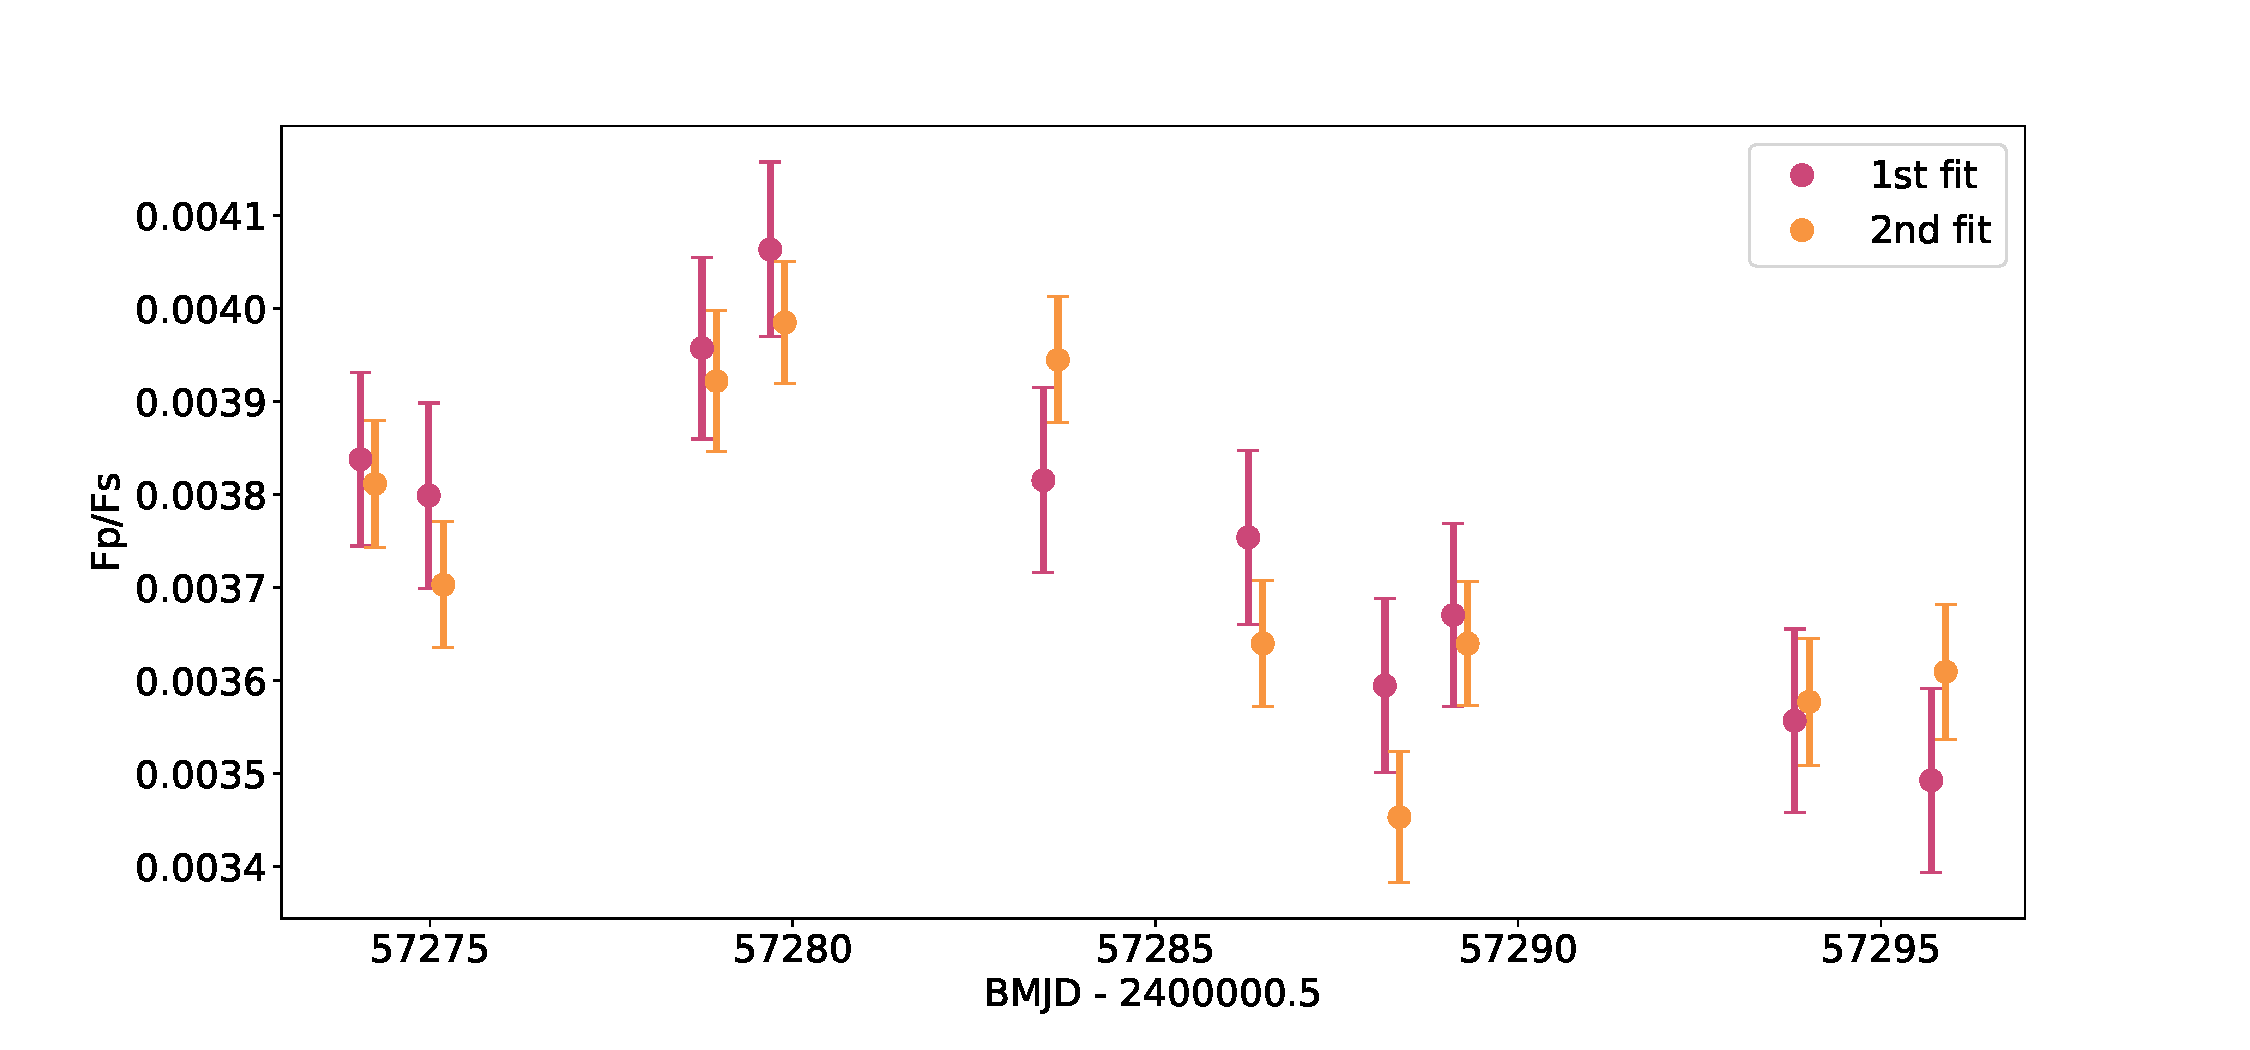
\includegraphics[width=\linewidth]{Wasp18b_EclipseDepths1stv2nd.pdf}
    \caption{Measured eclipse depths of WASP-18b over time in orange, for the ten semi-consecutive eclipses. Pink shows the eclipse depths from the first fit, where all parameters are free. Orange show the eclipse depths from the second fit, where the orbital distance, inclination and \nth{2} order quadratic term are fixed to the weighted mean from the first fit.}
    \label{P3:app:depths}
\end{sidewaysfigure}

\begin{figure}
    \centering
    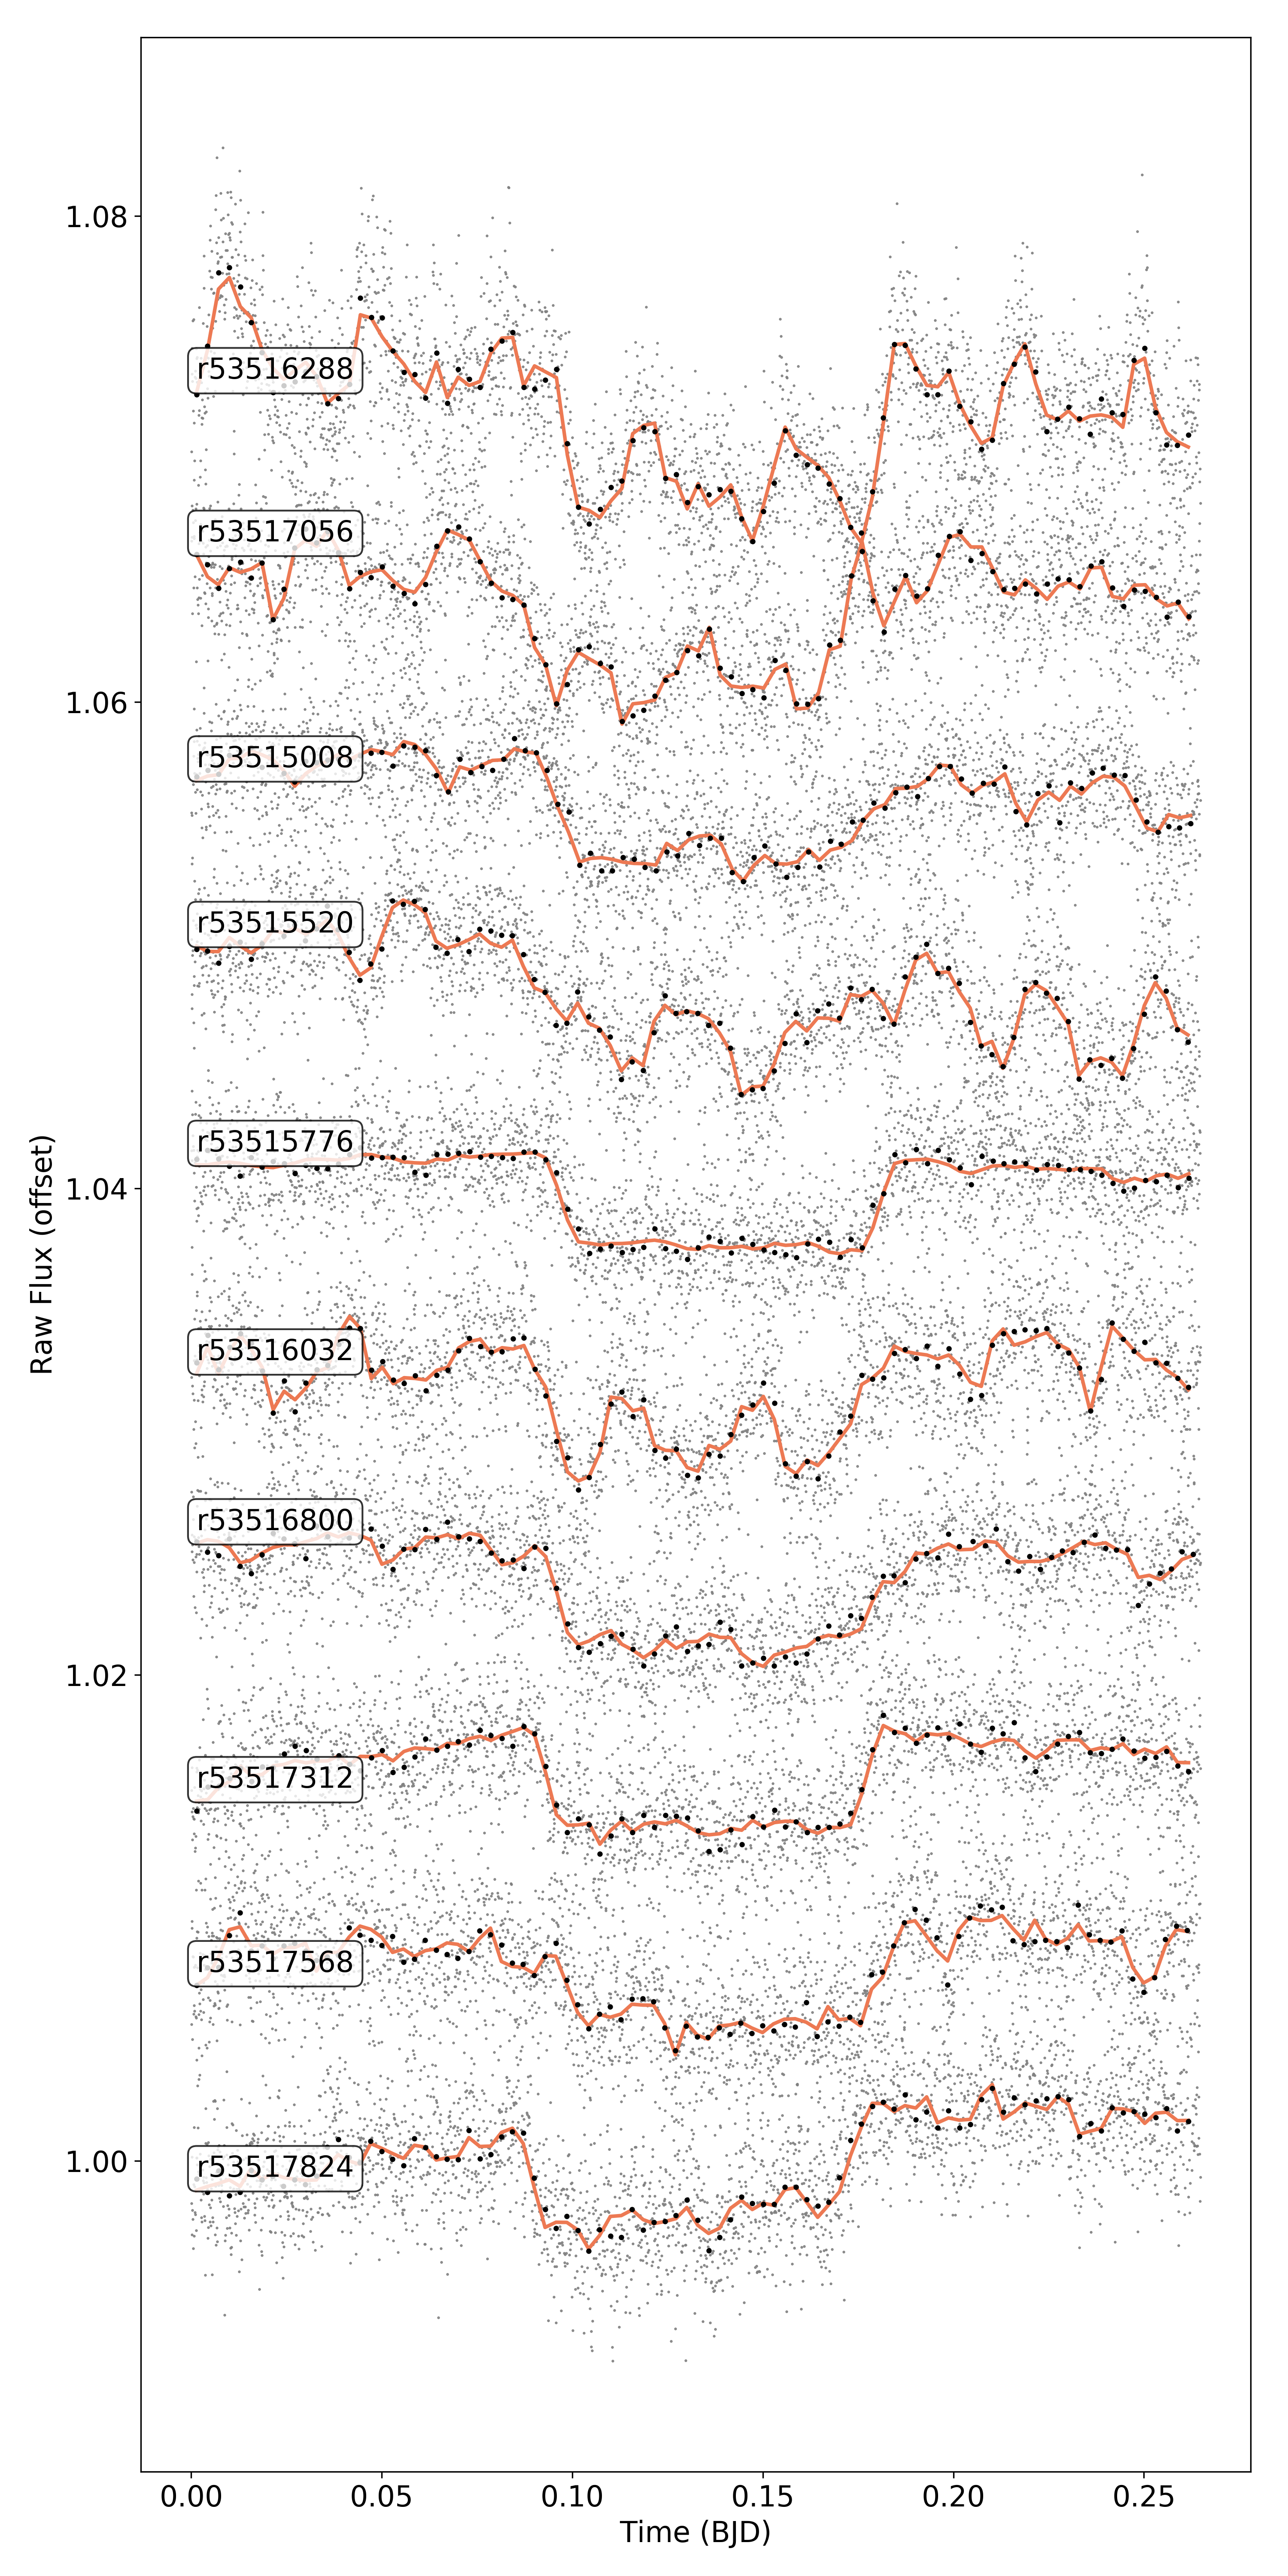
\includegraphics[height=\textheight]{Rawlightcurves_W18b.png}
    \caption{Raw eclipse lightcurves of WASP-18b with best fit systematic and eclipse model in orange.}
    \label{P3:fig:rawlcs}
\end{figure}

\begin{figure}
    \centering
    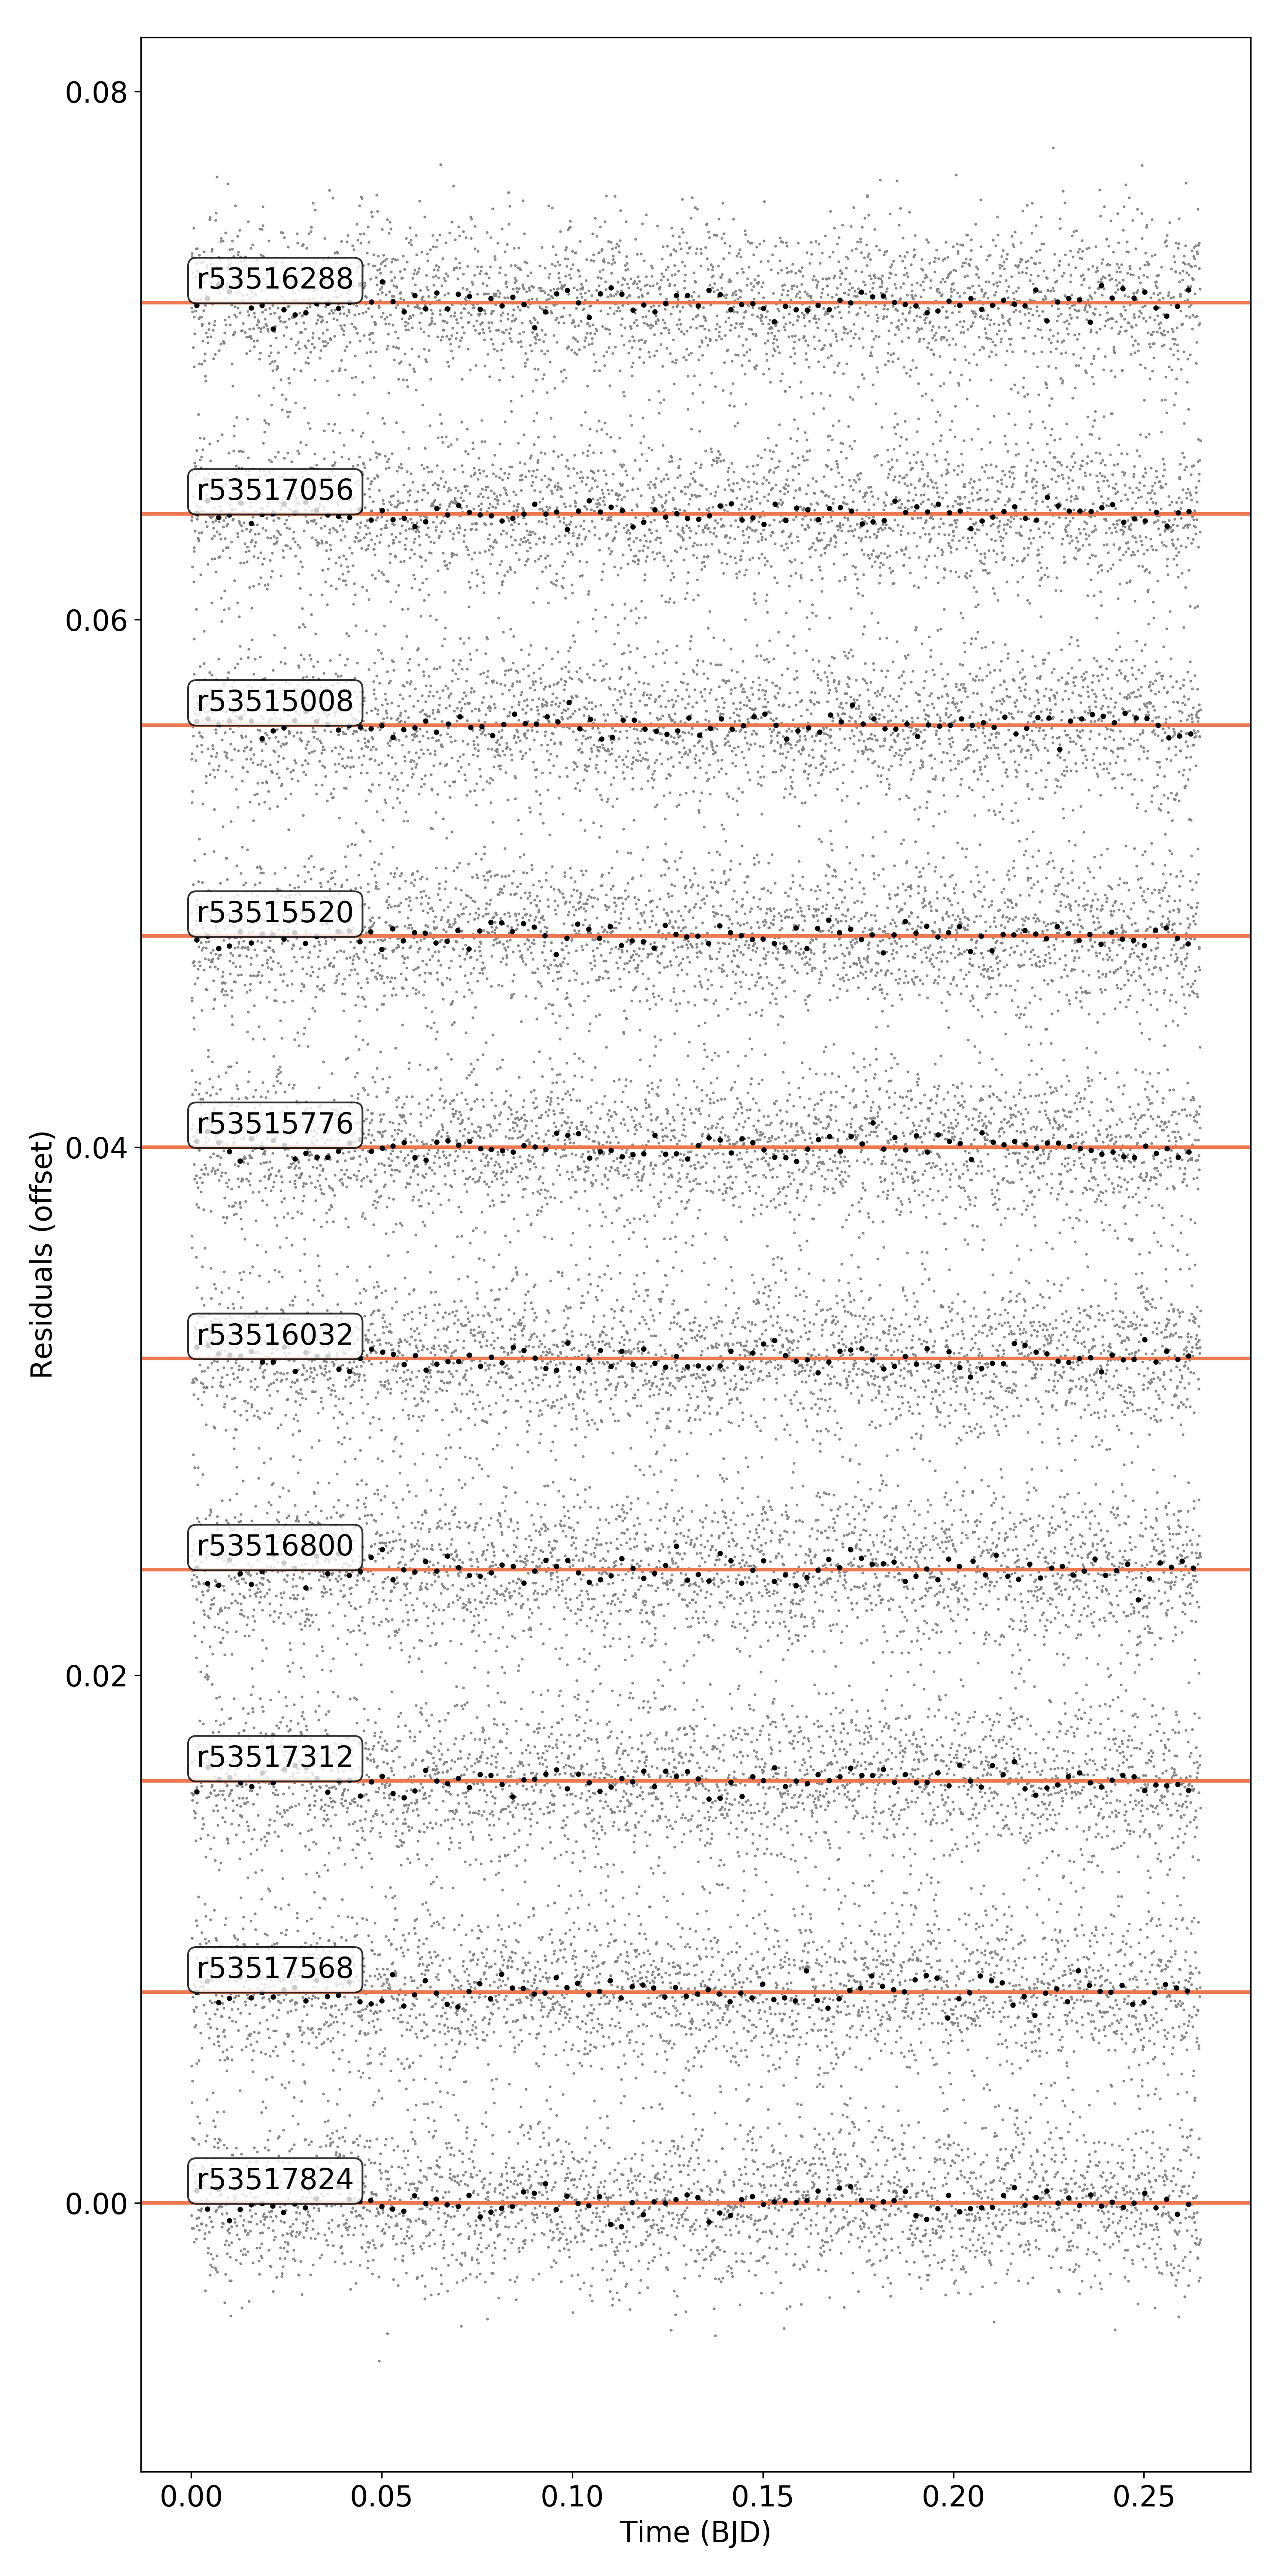
\includegraphics[height=\textheight]{Residuals_W18b.png}
    \caption{Residuals of WASP-18b eclipses with best fit systematic and eclipse model subtracted.}
    \label{P3:fig:residuallcs}
\end{figure}

\end{subappendices}
